\documentclass[11pt]{charter}

% El títulos de la memoria, se usa en la carátula y se puede usar el cualquier lugar del documento con el comando \ttitle
\titulo{Sistema de monitoreo en tiempo real para el adulto mayor} 

% Nombre del posgrado, se usa en la carátula y se puede usar el cualquier lugar del documento con el comando \degreename
\posgrado{Carrera de Especialización en Sistemas Embebidos} 
%\posgrado{Carrera de Especialización en Internet de las Cosas} 
%\posgrado{Carrera de Especialización en Intelegencia Artificial}
%\posgrado{Maestría en Sistemas Embebidos} 
%\posgrado{Maestría en Internet de las cosas}

% Tu nombre, se puede usar el cualquier lugar del documento con el comando \authorname
\autor{William's Ernesto Limonchi Sandoval} 

% El nombre del director y co-director, se puede usar el cualquier lugar del documento con el comando \supname y \cosupname y \pertesupname y \pertecosupname
\director{Lucas Dórdolo}
\pertenenciaDirector{Director del trabajo} 
% FIXME:NO IMPLEMENTADO EL CODIRECTOR ni su pertenencia
\codirector{} % si queda vacio no se deberíá incluir 
\pertenenciaCoDirector{}

% Nombre del cliente, quien va a aprobar los resultados del proyecto, se puede usar con el comando \clientename y \empclientename
\cliente{Javier Vasquez de Velasco}
\empresaCliente{Especialista Ferreyros}

% Nombre y pertenencia de los jurados, se pueden usar el cualquier lugar del documento con el comando \jurunoname, \jurdosname y \jurtresname y \perteunoname, \pertedosname y \pertetresname.
\juradoUno{Nombre y Apellido (1)}
\pertenenciaJurUno{pertenencia (1)} 
\juradoDos{Nombre y Apellido (2)}
\pertenenciaJurDos{pertenencia (2)}
\juradoTres{Nombre y Apellido (3)}
\pertenenciaJurTres{pertenencia (3)}
 
\fechaINICIO{13 de octubre de 2020}		%Fecha de inicio de la cursada de GdP \fechaInicioName
\fechaFINALPlanificacion{11 de diciembre de 2020} 	%Fecha de final de cursada de GdP
\fechaFINALTrabajo{22 de agosto de 2021}		%Fecha de defensa pública del trabajo final


\begin{document}

\maketitle
\thispagestyle{empty}
\pagebreak


\thispagestyle{empty}
{\setlength{\parskip}{0pt}
\tableofcontents{}
}
\pagebreak


\section{Registros de cambios}
\label{sec:registro}


\begin{table}[ht]
\label{tab:registro}
\centering
\begin{tabularx}{\linewidth}{@{}|c|X|c|@{}}
\hline
\rowcolor[HTML]{C0C0C0} 
Revisión & \multicolumn{1}{c|}{\cellcolor[HTML]{C0C0C0}Detalles de los cambios realizados} & Fecha      \\ \hline
1.0      & Creación del documento                                          & 23/10/2020 \\ \hline
1.1      & Presentación hasta el punto 6                                   & 06/11/2020 \\ \hline
1.2      & Correcciones de Practico 1                                      & 15/11/2020 \\ \hline
1.3      & Correcciones de Practico 2                                      & 24/11/2020 \\ \hline
1.4      & Correcciones de Practico 3                                      & 25/11/2020 \\ \hline
1.5      & Presentación completa                                           & 27/11/2020 \\ \hline
%		   Con texto partido \newline
%		   En varias líneas \newline
%		   A propósito                                                     & dd/mm/aaaa \\ \hline
\end{tabularx}
\end{table}

\pagebreak



\section{Acta de constitución del proyecto}
\label{sec:acta}

\begin{flushright}
Buenos Aires, \fechaInicioName
\end{flushright}

\vspace{2cm}

Por medio de la presente se acuerda con el Ing. \authorname\hspace{1px} que su Trabajo Final de la \degreename\hspace{1px} se titulará ``\ttitle'', consistirá esencialmente en observar la temperatura, nivel de saturación de oxígeno y detectar caída del adulto mayor en tiempo real, y tendrá un presupuesto preliminar estimado de 611 hs de trabajo con fecha de inicio \fechaInicioName\hspace{1px} y fecha de presentación pública \fechaFinalName.

Se adjunta a esta acta la planificación inicial.

\vfill

% Esta parte se construye sola con la información que hayan cargado en el preámbulo del documento y no debe modificarla
\begin{table}[ht]
\centering
\begin{tabular}{ccc}
\begin{tabular}[c]{@{}c@{}}Ariel Lutenberg \\ Director posgrado FIUBA\end{tabular} & \hspace{2cm} & \begin{tabular}[c]{@{}c@{}}\clientename \\ \empclientename \end{tabular} \vspace{2.5cm} \\ 
\multicolumn{3}{c}{\begin{tabular}[c]{@{}c@{}} \supname \\ Director del Trabajo Final\end{tabular}} \vspace{2.5cm} \\
%\begin{tabular}[c]{@{}c@{}}\jurunoname \\ Jurado del Trabajo Final\end{tabular}     &  & \begin{tabular}[c]{@{}c@{}}\jurdosname\\ Jurado del Trabajo Final\end{tabular}  \vspace{2.5cm}  \\
%\multicolumn{3}{c}{\begin{tabular}[c]{@{}c@{}} \jurtresname\\ Jurado del Trabajo Final\end{tabular}} \vspace{.5cm}                                                                     
\end{tabular}
\end{table}




\section{Descripción técnica-conceptual del proyecto a realizar}
\label{sec:descripcion}

\begin{consigna}{black}
El 30 de enero de 2020, la OMS declaró la epidemia de COVID-19, esta enfermedad respiratoria provoca mayor mortalidad en personas mayores de 60 años. Una medida que han adoptado todos los países ha sido el distanciamiento social lo que genera que las familias estén lejos de sus familiares más adultos, además de desconocer el estado de salud de sus seres queridos. 

El objetivo del sistema a desarrollar es conocer el nivel de temperatura, el nivel de saturación de oxígeno en la sangre y si adulto mayor ha sufrido alguna caída. El microcontrolador obtiene toda esta data mediante los diferentes sensores para luego procesar y almacenar la información en un memoria micro SD. Asimismo, esta información es transmitida mediante un módulo Wifi hacia una plataforma Web en la que el usuarios o los usuarios puedan observar la data obtenida. 

El presente proyecto se destaca especialmente por incorporar un sistema en tiempo real por lo que se monitorea y notifica, de presentarse alguna eventualidad, de la manera más rápida y óptima. 

En la Figura 1 se muestra el diagrama de bloques del sistema. Se observa el microcontrolador con cada uno de los sensores del sistema, así como  el módulo de alimentación que será una batería y por último, el Wifi que transmite la información hacía la página web.

\vspace{25px}

\begin{figure}[htpb]
\centering 
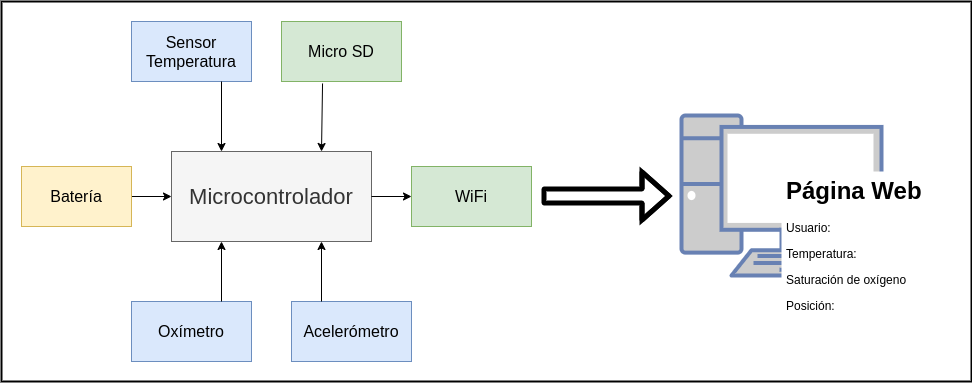
\includegraphics[width=1\textwidth]{./Figuras/diagBloques.png}
\caption{Diagrama en bloques del sistema}
\label{fig:diagBloques}
\end{figure}


\end{consigna}


\section{Identificación y análisis de los interesados}
\label{sec:interesados}

\begin{consigna}{black} 
\vspace{-35px}
\begin{itemize}
\item Auspiciante: es riguroso y exigente con la rendición de gastos y en el desarrollo del proyecto en el tiempo establecido.
\item Cliente: Javier Vasquez de Velasco, interesado en el desarrollo del proyecto para utilizarlo en el monitoreo de su madre que padece de una enfermedad.
\item Opositor: Wok Solución, empresa que desarrolla equipos de monitoreo y videovigilancia.
\end{itemize}

\begin{table}[ht]
%\caption{Identificación de los interesados}
%\label{tab:interesados}
\begin{tabularx}{\linewidth}{@{}|l|X|X|l|@{}}
\hline
\rowcolor[HTML]{000000} 
Rol           & Nombre y Apellido & Organización 	& Puesto 	\\ \hline
Auspiciante   & Williams Limonchi Falen & - 		& Mecánico	\\ \hline
Cliente       & \clientename     &\empclientename	& Ing. Mecánico	\\ \hline
Responsable   & \authorname       & FIUBA        	& Alumno 	\\ \hline
Colaboradores & -                 & -             	& -       	\\ \hline
Orientador    & \supname	      & \pertesupname 	& Director	Trabajo final \\ \hline
Equipo        & - \newline 
				-          & -            	& -       	\\ \hline
Opositores    & Wok Solución      & -            	& -      	\\ \hline
Usuario final & Adultos mayores   & -              	& -      	\\ \hline
\end{tabularx}
\end{table}


\end{consigna}



\section{1. Propósito del proyecto}
\label{sec:proposito}

\begin{consigna}{black}
El propósito de este proyecto es desarrollar un prototipo de monitoreo en tiempo real de un adulto mayor. Este desarrollo permite visualizar el estado de temperatura, saturación de oxígeno y si el adulto mayor ha sufrido alguna caída. Además de notificar por si ocurre alguna eventualidad a los familiares. 

\end{consigna}

\section{2. Alcance del proyecto}
\label{sec:alcance}

\begin{consigna}{black}
Para la realización de este trabajo se llevará a cabo el diseño e implementación del hardware junto al desarrollo del firmware del prototipo del proyecto el cual correrá en un sistema de tiempo real. 

El presente proyecto incluye la adquisición de datos de los sensores de temperatura, saturación de oxígeno y acelerómetro. También incluye el procesamiento de información, almacenamiento de la data en tarjeta micro SD y transmisión de datos mediante WiFi hacia una plataforma Web. Además, se desarrollará una plataforma Web en la cual se visualizarán los datos obtenidos del sistema y notificará a los usuarios de producirse algún evento de caída.   

El presente proyecto no incluye un diagnóstico o análisis de los datos recolectados para determinar el estado del adulto mayor.

\end{consigna}


\section{3. Supuestos del proyecto}
\label{sec:supuestos}

\begin{consigna}{black}
Para el desarrollo del presente proyecto se supone que:

\begin{itemize}
\item Se contará con una CIAA, STM32 u otra placa similar a definir. 
\item Se contará con 2 juegos de sensores y actuadores.
\item Se contará con los componentes electrónicos necesarios para la implementación del prototipo.
\item Se dispondrá de las 600hs requeridas para realizar el proyecto. 
\end{itemize}

\end{consigna}

\section{4. Requerimientos}
\label{sec:requerimientos}

\begin{consigna}{black}
\vspace{-35px}
\begin{enumerate}
\item Requerimientos del sistema
	\begin{enumerate}
	\item El proyecto debe utilizar un sistema operativo en tiempo real.
	\item El sistema debe enviar la información cada 1 segundo.
	\item El sistema debe tomar 1000 muestras del sensor de saturación de oxígeno en un periodo de 1 segundo.
	\item El sistema debe tomar 2 muestras del sensor de temperatura en cada 1 segundo. 
	\item El sistema debe incorporar un algoritmo de detección de caídas.
	\item El sistema debe transmitir la información mediante un módulo WiFi hacia una plataforma Web, utilizando el protocolo MQTT.
	\item El sistema debe operar con batería que dure al menos 12 horas.
	\item El sistema debe tener la capacidad de almacenamiento de datos recolectados por al menos un mes. 
	\item El sistema debe tener como prioridad la detección de caídas, además de enviar esta información en un tiempo menor a 100 ms.
	\item El sistema debe utilizar GIT para el control de versiones.
	\end{enumerate}
\item Requerimiento de la plataforma Web
	\begin{enumerate}
	\item La plataforma Web debe mostrar la información, estados y valores de los sensores en un tiempo entre 100 y 200ms.
	\item La plataforma Web debe notificar valores medidos fuera de rango o si se presenta un evento de caída.
	\item La plataforma Web debe permitir la modificación de parámetros de la información del usuario.
	\end{enumerate}
\item Requerimiento de Testing 
	\begin{enumerate}
	\item Test unitario de cada función de software.
	\item Test de detección de caídas.
	\item Test de duración de batería.
	\item Test de almacenamiento de información.
	\end{enumerate}
\item Requerimiento de documentación
	\begin{enumerate}
	\item El desarrollo estará acompañado por una memoria técnica.
	\item El desarrollo estará acompañado de guía de usuario.
	\end{enumerate}

\end{enumerate}
\end{consigna}
\vspace{-15px}
\section{Historias de usuarios (\textit{Product backlog})}
\label{sec:backlog}

\begin{consigna}{black}
\vspace{-35px}
\begin{itemize}
\item Como adulto mayor, quiero poder seleccionar fechas para visualizar el estado de salud por día y hora. (\textit{Story Points: 7})
\item Como familiar del adulto mayor, quiero poder descargar la información para llevarlo a algún centro de salud. (\textit{Story Points: 9}) 
\item Como familiar del adulto mayor, quiero que me notifiquen cada cierto tiempo para conocer el estado de salud de mi familiar. (\textit{Story Points: 9}) 
\item Como adulto mayor, quiero una alerta para conocer si el dispositivo no está conectado a internet.(\textit{Story Points: 9})  
\item Como adulto mayor, quiero que me notifiquen cuando la batería esté en 15\% para recargar la batería.(\textit{Story Points: 6}) 
\end{itemize}
\end{consigna}
\vspace{-15px}
\section{5. Entregables principales del proyecto}
\label{sec:entregables}

\begin{consigna}{black}
\vspace{-35px}
\begin{itemize}
\item Prototipo del sistema.
\item Manual de usuario.
\item Diagrama esquemático.
\item Código fuente.
\item Informe final.

\end{itemize}

\end{consigna}
\vspace{-10px}
\section{6. Desglose del trabajo en tareas}
\label{sec:wbs}

\begin{consigna}{black}
\vspace{-35px}
\begin{enumerate}
\item Análisis preliminar (37 hs)
	\begin{enumerate}
	\item Investigación bibliográfica. (20 hs)
	\item Definir componentes a utilizar.  (12 hs)
	\item Elección de microcontrolador. (5 hs)
	\end{enumerate}
\item Diseño general del proyecto (35 hs)
	\begin{enumerate}
	\item Realización de diagrama de bloques. (4 hs)
	\item Realización de diseño de la arquitectura del sistema. (4 hs)
	\item Obtener los componentes para el prototipo de pruebas. (12 hs)
	\item Diagrama de flujo del programa. (15 hs)	
	\end{enumerate}
\item Diseño de Hardware (61 hs)
	\begin{enumerate}
	\item Elaborar el diagrama esquemático del prototipo. (20 hs)
	\item Realizar pruebas del circuito del prototipo. (15 hs)
	\item Elaborar el PCB del prototipo de pruebas. (20 hs)
	\item Montar el prototipo de pruebas. (3 hs)
	\item Verificar conexiones de la PCB. (3 hs)
	\end{enumerate}
\item Diseño de Firmware (165 hs)
	\begin{enumerate}
	\item Desarrollo del sistema de lectura de los sensores de temperatura y saturación.(25 hs)
	\item Desarrollo del sistema de lecturas del acelerómetro. (25 hs)
	\item Desarrollo del sistema de almacenamiento de datos. (20 hs)
	\item Desarrollo del sistema de transmisión de datos. (20 hs)
	\item Desarrollo del sistema de monitoreo de tensión de la batería. (15 hs)
	\item Desarrollo del sistema en RTOS. (40 hs)
	\item Realizar pruebas de los sistemas en conjunto. (20 hs)
	\end{enumerate}
\item Desarrollo de la aplicación Web (65 hs)
	\begin{enumerate}
	\item Investigar el lenguaje de programación más apropiado para desarrollar una aplicación Web. (15 hs)
	\item Diseño de mock-ups de la aplicación. (10 hs)
	\item Desarrollo de la aplicación Web. (40 hs)
	\end{enumerate}
\item Implementación del prototipo (30 hs)
	\begin{enumerate}
	\item Elaborar la PCB del prototipo del proyecto final. (20 hs)
	\item Montar el proyecto. (6 hs)
	\item Verificar conexiones de la PCB. (4 hs)
	\end{enumerate}
\item Testing y depuración (193 hs)
	\begin{enumerate}
	\item Registrar las pruebas realizadas. (3 hs)
	\item Realizar pruebas de los sistemas. (30 hs)
	\item Realizar pruebas de comunicación. (30 hs)
	\item Realizar pruebas de detección de caídas. (30hs)
	\item Realizar pruebas de duración de batería. (20hs)
	\item Realizar pruebas de almacenamiento de información. (20hs)
	\item Realizar pruebas de la aplicación web.  (30 hs)
	\item Testear el sistema en conjunto. (30 hs)
	\end{enumerate}
\item Documentación (24 hs)
	\begin{enumerate}
	\item Elaborar el manual para el desarrollador. (15 hs)
	\item Elaborar el manual de usuario. (9 hs)
	\end{enumerate}
\item Presentación del trabajo (65 hs)
	\begin{enumerate}
	\item Elaborar la memoria técnica del trabajo final (40 hs)
	\item Elaborar la presentación del trabajo final (25 hs)
	\end{enumerate}
\end{enumerate}

Cantidad total de horas: (675 hs)

\end{consigna}

\newpage
\section{7. Diagrama de Activity On Node}
\label{sec:AoN}

\begin{consigna}{black} 

%La figura \ref{fig:AoN} fue elaborada con el paquete latex tikz y pueden consultar la siguiente referencia \textit{online}:

%\url{https://www.overleaf.com/learn/latex/LaTeX_Graphics_using_TikZ:_A_Tutorial_for_Beginners_(Part_3)\%E2\%80\%94Creating_Flowcharts}
\vspace{-15px}
\begin{figure}[!htpb]
\centering 
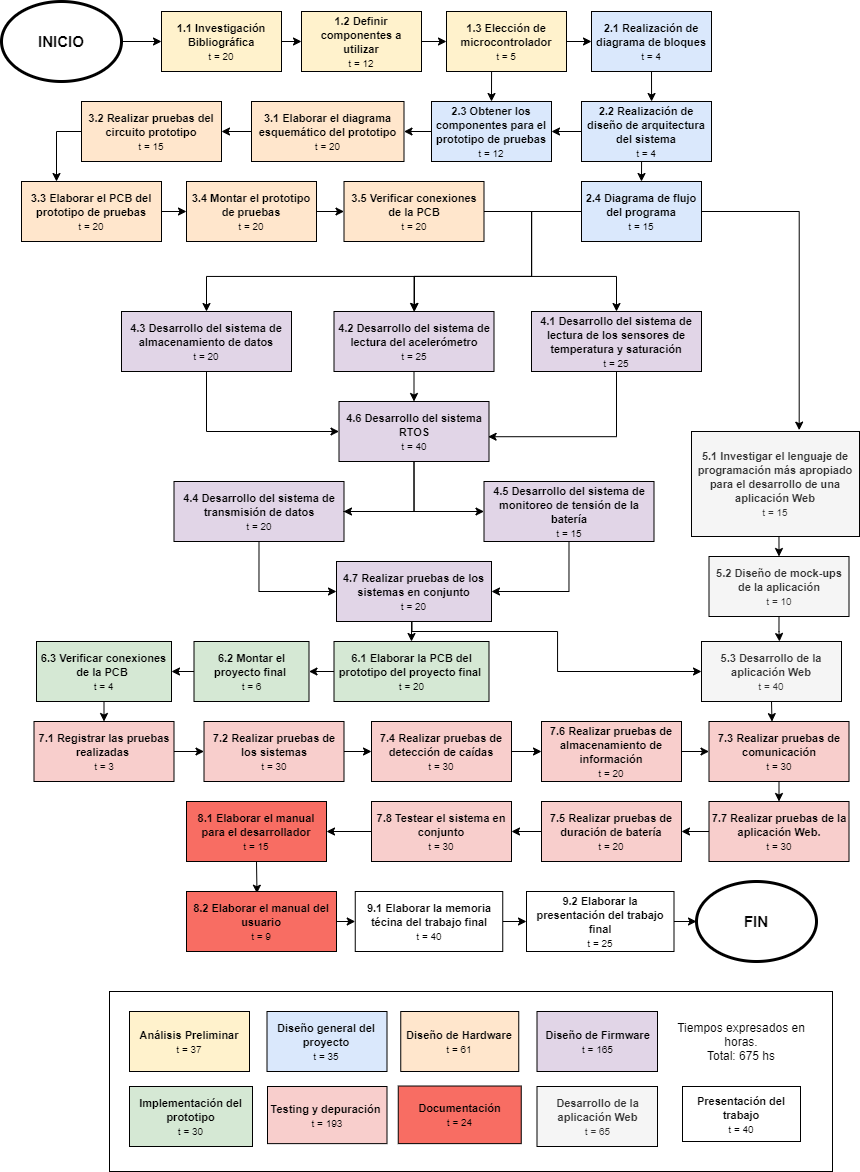
\includegraphics[width=1\textwidth]{./Figuras/AoN.png}
\caption{Diagrama en \textit{Activity on Node}}
\label{fig:AoN}
\end{figure}

\end{consigna}

\section{8. Diagrama de Gantt}
\label{sec:gantt}
\vspace{-10px}
\begin{consigna}{black}
Para el diagrama de Gantt se consideró una dedicación parcial promedio de 2 hs durante todos los días hábiles.

\begin{figure}[htpb]
\centering 
\centering 
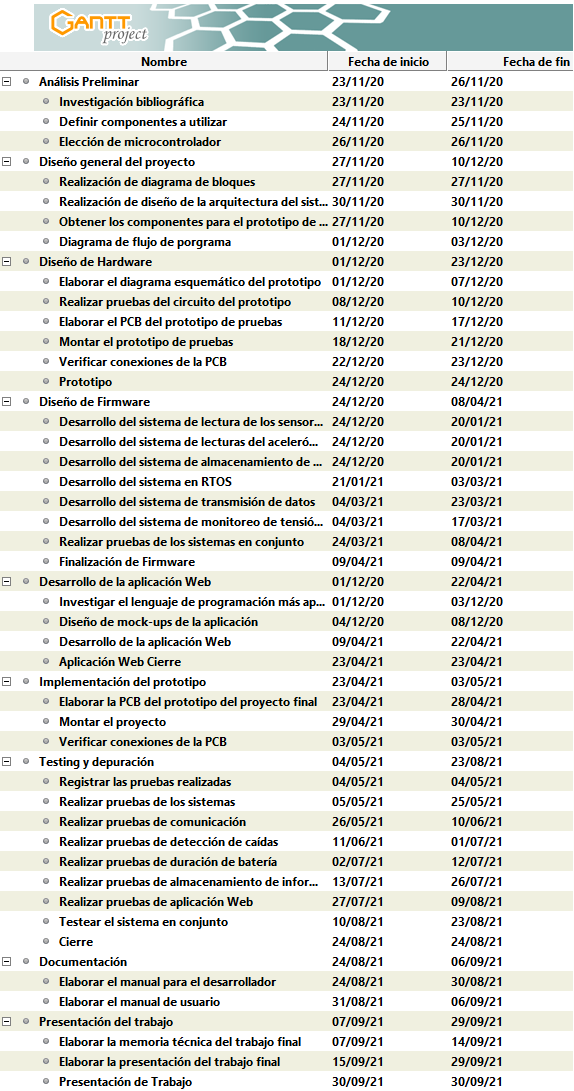
\includegraphics[width=0.60\textwidth]{./Figuras/DiagramaGantt_Nombres.png}
\caption{Diagrama en gantt desarrollado en \textit{Gantt Project}}
\label{fig:gantt1}
\end{figure}
\vspace{-25px}
\begin{figure}[!htpb]
\centering 
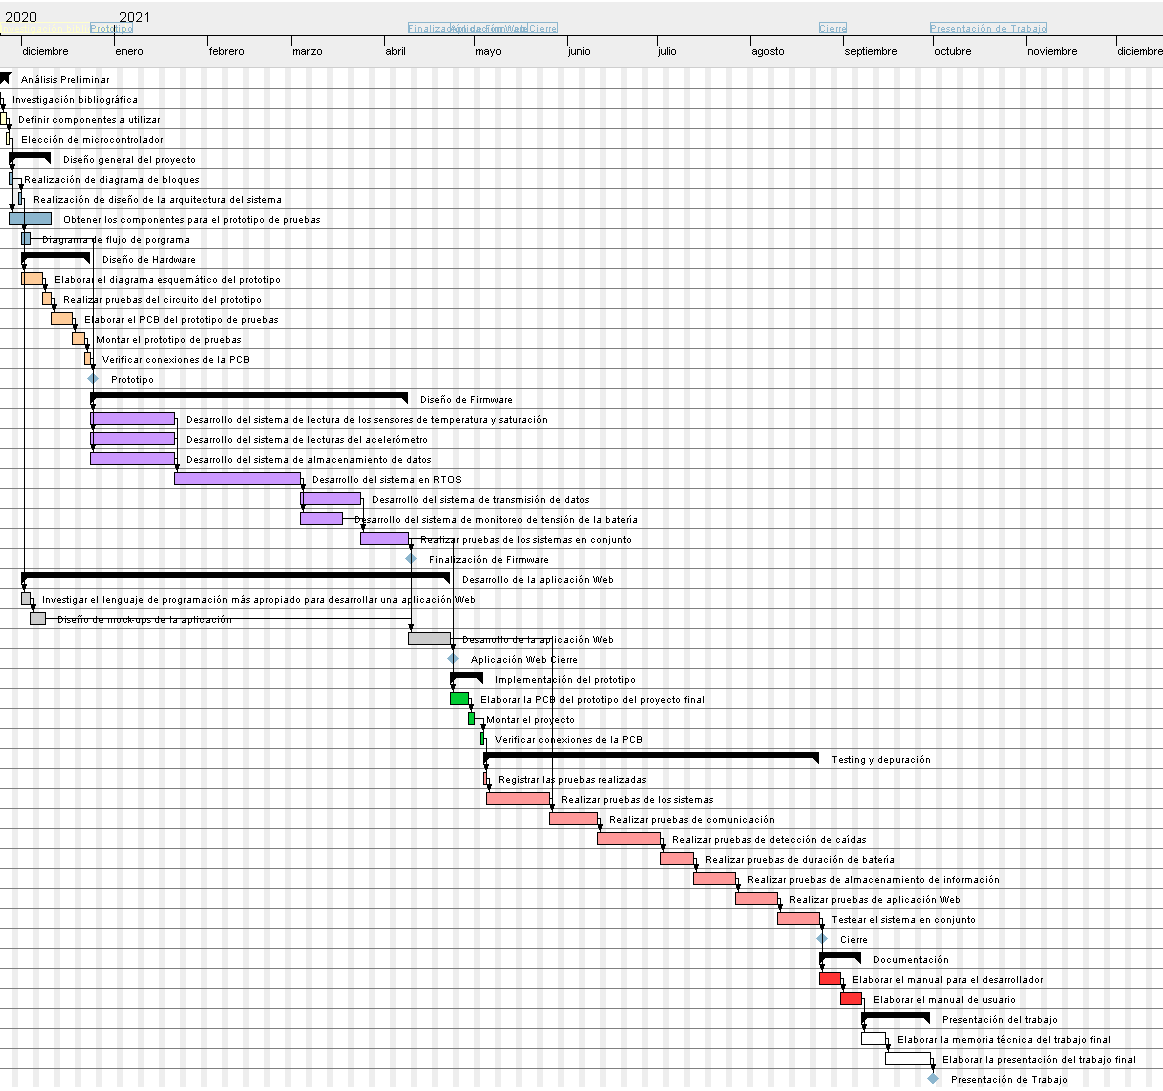
\includegraphics[width=1\textwidth]{./Figuras/DiagramaGantt_Eventos.png}
\caption{Diagrama en gantt desarrollado en \textit{Gantt Project}}
\label{fig:gantt2}
\end{figure}

\end{consigna}
\vspace{30px}
\section{9. Matriz de uso de recursos de materiales}
\label{sec:recursos}
%\vspace{-300px}
\begin{table}[!hbt]
\label{tab:recursos}
%\centering
%\resizebox*{1\textwidth}{!}{
\begin{tabularx}{\linewidth}{@{}|c|X|c|c|c|@{}}
\hline
\cellcolor[HTML]{C0C0C0} & \cellcolor[HTML]{C0C0C0} & \multicolumn{3}{c|}{\cellcolor[HTML]{C0C0C0}Recursos requeridos (horas)} \\ \cline{3-5} 
\multirow{-2}{*}{\cellcolor[HTML]{C0C0C0}\begin{tabular}[c]{@{}c@{}}Código\\ WBS\end{tabular}} & 
\multirow{-2}{*}{\cellcolor[HTML]{C0C0C0}\begin{tabular}[c]{@{}c@{}}Nombre de la tarea\end{tabular}} & PC & Placa de desarrollo & Sensores \\ \hline
 1.  & Análisis Preliminar & 37 & &  \\ \hline
 2.  & Diseño general del proyecto & 35 &  & \\ \hline
 3.1  & Elaborar el diagrama esquemático del prototipo & 20 &  & \\ \hline 
 3.2  & Realizar pruebas del circuito prototipo & 15  &  & \\ \hline
 3.3  & Elaborar el PCB del prototipo de prueba & 20 &  & \\ \hline
 3.4  & Montar el prototipo de pruebas & & 10 & 10  \\ \hline
 3.5  & Verificar conexiones del PCB & & 10 & 10   \\ \hline
 4.1  & Desarrollo del sistema de lectura de los sensores de temperatura y saturación & 20 &  &    \\ \hline
 4.2  & Desarrollo del sistema de lectura del acelerómetro & 25 & &   \\ \hline
 4.3  & Desarrollo del sistema de almacenamiento de datos & 25 &  &    \\ \hline
 4.4  & Desarrollo del sistema de transmisión de datos & 20 &  &    \\ \hline
 4.5  & Desarrollo del sistema de monitoreo de tensión de la batería & 15  &  &   \\ \hline
 4.6  & Desarrollo del sistema RTOS & 40  &  &  \\ \hline
 4.7  & Realizar pruebas de los sistemas en conjunto & 20 &  &   \\ \hline
 5.1  & Investigar el lenguaje de programación más apropiado para el desarrollo de una aplicación Web & 15 &  &   \\ \hline 
 5.2  & Diseño de mock-ups de la aplicación & 10  &  &  \\ \hline
 5.3  & Desarrollo de la aplicación Web & 40 &  &  \\ \hline
 6.1  & Elaborar la PCB del prototipo del proyecto final & 20 & &  \\ \hline
 6.2  & Montar el proyecto final &  & 3 & 3 \\ \hline
 6.3  & Verificar conexiones de la PCB &  & 2 & 2  \\ \hline
 7.1  & Registrar las pruebas realizadas & 4 &  &  \\ \hline
 7.2  & Realizar pruebas de los sistemas & 10  & 10 & 10 \\ \hline
 7.3  & Realizar pruebas de comunicación & 10 & 10 & 10  \\ \hline
 7.4  & Realizar pruebas de detección de caídas & 10 & 10 & 10  \\ \hline
 7.5  & Realizar pruebas de duración de batería & 5 & 5  & 10  \\ \hline 
 7.6  & Realizar pruebas de almacenamiento de información & 5 & 5  & 10  \\ \hline 
 7.7  & Realizar pruebas de la aplicación Web & 20 & 5 & 5 \\ \hline 
 7.8  & Testear el sistema en conjunto & 10 & 10 & 10 \\ \hline 
 8.  & Documentación & 24 &  &   \\ \hline
 9.  & Presentación del trabajo & 65 &  &   \\ \hline 
\end{tabularx}
\end{table}
%\vspace{30px}

\section{10. Presupuesto detallado del proyecto}
\label{sec:presupuesto}
\vspace{-10px}
\begin{consigna}{black}
La moneda utilizada en el presupuesto es el dólar.
\end{consigna}
\begin{table}[htpb]
\centering
\begin{tabularx}{\linewidth}{@{}|X|c|r|r|@{}}
\hline
\rowcolor[HTML]{C0C0C0} 
\multicolumn{4}{|c|}{\cellcolor[HTML]{C0C0C0}COSTOS DIRECTOS} \\ \hline
\rowcolor[HTML]{C0C0C0} 
Descripción &
  \multicolumn{1}{c|}{\cellcolor[HTML]{C0C0C0}Cantidad} &
  \multicolumn{1}{c|}{\cellcolor[HTML]{C0C0C0}Valor unitario} &
  \multicolumn{1}{c|}{\cellcolor[HTML]{C0C0C0}Valor total} \\ \hline
Mano de obra  &
  \multicolumn{1}{c|}{675} &
  \multicolumn{1}{c|}{\$ 5.00} &
  \multicolumn{1}{c|}{\$ 2700.00} \\ \hline
Tarjeta STM 32  &
  \multicolumn{1}{c|}{1} &
  \multicolumn{1}{c|}{\$ 50.00} &
  \multicolumn{1}{c|}{\$ 50.00} \\ \hline
Sensor MAX30105 &
  \multicolumn{1}{c|}{2} &
  \multicolumn{1}{c|}{\$ 10.00} &
  \multicolumn{1}{c|}{\$ 20.00} \\ \hline
Sensor LM35 &
  \multicolumn{1}{c|}{2} &
  \multicolumn{1}{c|}{\$ 1.00} &
  \multicolumn{1}{c|}{\$ 2.00} \\ \hline
ADXL355 &
  \multicolumn{1}{c|}{2} &
  \multicolumn{1}{c|}{\$ 5.00} &
  \multicolumn{1}{c|}{\$ 10.00} \\ \hline
ESP8266 &
  \multicolumn{1}{c|}{2} &
  \multicolumn{1}{c|}{\$ 7.00} &
  \multicolumn{1}{c|}{\$ 14.00} \\ \hline
PCB &
  \multicolumn{1}{c|}{2} &
  \multicolumn{1}{c|}{\$ 30.00} &
  \multicolumn{1}{c|}{\$ 60.00} \\ \hline
Otros componentes &
  \multicolumn{1}{c|}{1} &
  \multicolumn{1}{c|}{\$ 30.00} &
  \multicolumn{1}{c|}{\$ 30.00} \\ \hline
\multicolumn{3}{|c|}{SUBTOTAL} &
  \multicolumn{1}{c|}{\$ 2886.00} \\ \hline
\rowcolor[HTML]{C0C0C0} 
\multicolumn{4}{|c|}{\cellcolor[HTML]{C0C0C0}COSTOS INDIRECTOS} \\ \hline
\rowcolor[HTML]{C0C0C0} 
Descripción &
  \multicolumn{1}{c|}{\cellcolor[HTML]{C0C0C0}Cantidad} &
  \multicolumn{1}{c|}{\cellcolor[HTML]{C0C0C0}Valor unitario} &
  \multicolumn{1}{c|}{\cellcolor[HTML]{C0C0C0}Valor total} \\ \hline
30\% de costos directos &
  \multicolumn{1}{c|}{1} &
  \multicolumn{1}{c|}{\$ 865.80} &
  \multicolumn{1}{c|}{\$ 865.80} \\ \hline
\multicolumn{3}{|c|}{SUBTOTAL} &
  \multicolumn{1}{c|}{} \\ \hline
\rowcolor[HTML]{C0C0C0}
\multicolumn{3}{|c|}{TOTAL} & \$ 3751.00
   \\ \hline
\end{tabularx}%
\end{table}
\vspace{10px}


\section{11. Matriz de asignación de responsabilidades}
\label{sec:responsabilidades}
\vspace{-10px}
\begin{consigna}{black}

\begin{table}[!hbt]
\centering
\vspace{-20px}
\resizebox{1\textwidth}{!}{%
\begin{tabular}{@{}|c|l|c|c|c|c|@{}}
\hline
\rowcolor[HTML]{C0C0C0} 
\cellcolor[HTML]{C0C0C0} &
  \cellcolor[HTML]{C0C0C0} &
  \multicolumn{4}{c|}{\cellcolor[HTML]{C0C0C0}Listar todos los nombres y roles del proyecto} \\ \cline{3-6} 
\rowcolor[HTML]{C0C0C0} 
\cellcolor[HTML]{C0C0C0} &
  \cellcolor[HTML]{C0C0C0} &
  Responsable &
  Orientador &
  Equipo &
  Cliente \\ \cline{3-6} 
\rowcolor[HTML]{C0C0C0} 
\multirow{-3}{*}{\cellcolor[HTML]{C0C0C0}\begin{tabular}[c]{@{}c@{}}Código\\ WBS\end{tabular}} &
  \multirow{-3}{*}{\cellcolor[HTML]{C0C0C0}Nombre de la tarea} &
  Williams Limonchi &
  \supname &
  - &
  Javier Vasquez \\ \hline
 1.  & Análisis Preliminar & P & A & & I \\ \hline
 2.  & Diseño general del proyecto & P & A & & \\ \hline
 3.1  & Elaborar el diagrama esquemático del prototipo & P & I & & \\ \hline 
 3.2  & Realizar pruebas del circuito prototipo & P & I & & \\ \hline
 3.3  & Elaborar el PCB del prototipo de prueba & P & I & & \\ \hline
 3.4  & Montar el prototipo de pruebas & P & I & & \\ \hline
 3.5  & Verificar conexiones del PCB & P & I & &  \\ \hline
    &  & &  & &  \\ 
\multirow{-2}{*}{4.1} & \multirow{-2}{*}{\begin{tabular}[c]{@{}l@{}}Desarrollo del sistema de lectura de \\los sensores de temperatura y saturación\end{tabular}} & P & I/C & &  \\ \hline
 4.2  & Desarrollo del sistema de lectura del acelerómetro & P & I/C & &  \\ \hline
 4.3  & Desarrollo del sistema de almacenamiento de datos & P & I/C & &   \\ \hline
 4.4  & Desarrollo del sistema de transmisión de datos & P & I/C & &   \\ \hline
      &  & &  & &  \\ 
\multirow{-2}{*}{4.5} & \multirow{-2}{*}{\begin{tabular}[c]{@{}l@{}}Desarrollo del sistema de monitoreo de tensión\\de la batería\end{tabular}} & P & I/C & &  \\ \hline 
 4.6  & Desarrollo del sistema RTOS & P & I/C & & \\ \hline
 4.7  & Realizar pruebas de los sistemas en conjunto & P & I & &  \\ \hline
     &  & &  & &  \\ 
\multirow{-2}{*}{5.1} & \multirow{-2}{*}{\begin{tabular}[c]{@{}l@{}}Investigar el lenguaje de programación más \\apropiado para el desarrollo de una aplicación Web\end{tabular}} & P & I/C & &  \\ \hline 
 5.2  & Diseño de mock-ups de la aplicación & P & I & & \\ \hline
 5.3  & Desarrollo de la aplicación Web & P & I & & \\ \hline
 6.1  & Elaborar la PCB del prototipo del proyecto final & P & & &   \\ \hline
 6.2  & Montar el proyecto final & P &  & & \\ \hline
 6.3  & Verificar conexiones de la PCB & P & I & & I \\ \hline
 7.1  & Registrar las pruebas realizadas & P & I & & I \\ \hline
 7.2  & Realizar pruebas de los sistemas & P & I &  &  \\ \hline
 7.3  & Realizar pruebas de comunicación & P & I &  &  \\ \hline
 7.4  & Realizar pruebas de detección de caídas & P & I & &  \\ \hline
 7.5  & Realizar pruebas de duración de batería & P & I & &   \\ \hline 
 7.6  & Realizar pruebas de almacenamiento de información & P & I & &   \\ \hline 
 7.7  & Realizar pruebas de la aplicación Web & P & I & &  \\ \hline 
 7.8  & Testear el sistema en conjunto & P & I & & I \\ \hline 
 8.  & Documentación & P & I & & I \\ \hline
 9.  & Presentación del trabajo & P & I/A & & I \\ \hline 
\end{tabular}%
}
\end{table}

{\footnotesize
Referencias:
\begin{itemize}
	\item P = Responsabilidad Primaria
	\item S = Responsabilidad Secundaria
	\item A = Aprobación
	\item I = Informado
	\item C = Consultado
\end{itemize}
} %footnotesize
\end{consigna}
\vspace{-10px}
\section{12. Gestión de riesgos}
\label{sec:riesgos}
\vspace{-30px}
\begin{consigna}{black}
 
Riesgo 1: La placa NUCLEO 64-STM32 deja de funcionar.
\begin{itemize}
\item Severidad (S): 7\\
La severidad es moderada/alta, puesto si la placa deja de funcionar demoraría el inicio de las tareas 7.2, que consiste en la verificación del sistema.
\item Probabilidad de ocurrencia (O): 3\\
La probabilidad de ocurrencia es baja, además que se cuenta con una tarjeta extra para la realización de las tareas de verificación del sistema. 
\end{itemize}   

Riesgo 2: Las horas estimadas para la realización del proyecto sean menores a las reales.
\begin{itemize}
\item Severidad (9): La severidad es muy alta, puesto que se corre el riesgo de que no se alcance a presentar con puntualidad el proyecto. 
\item Ocurrencia (7): La probabilidad de ocurrencia es moderada/alta, el Responsable no posee experiencia en definir qué parte llevará un determinado tiempo. 
\end{itemize}

Riesgo 3: Disponibilidad de hardware. No se logra conseguir el hardware necesario.
\begin{itemize}
\item Severidad (9): No es posible adquirir el hardware (sensores, módulos, etc).
\item Ocurrencia (2): Existe una gran variedad de locales nacionales e internacionales que venden componentes electrónicos.
\end{itemize}

Riesgo 4: Error en fabricación de PCB. 
\begin{itemize}
\item Severidad (9): La severidad es muy alta, lo que implica que el sistema no funcione.
\item Ocurrencia (2): El diseño e implementación de la PCB no tiene un gran complejidad. Así como los componentes a montar en la PCB se fabrican en serie.
\end{itemize}

Riesgo 5: Pérdida o daño de los archivos del proyecto.
\begin{itemize}
\item Severidad (10): La severidad es muy alta, si se pierden los archivos del proyecto, el mismo se retrasaría.
\item Ocurrencia (3): Es poco probable, pero se utilizará un sistema de control de versiones para los archivos del proyecto.
\end{itemize}

Riesgo 6: No se realiza la comunicación inalámbrica entre el sistema y la aplicación Web.
\begin{itemize}
\item Severidad (9): La severidad es muy alta, si el sistema no logra realizar la comunicación no se visualizarían las mediciones.
\item Ocurrencia (4): Es probable, pero se utilizará servicios ya utilizados con anterioridad.
\end{itemize}

b) Tabla de gestión de riesgos:      (El RPN se calcula como RPN=SxO)
\begin{table}[htpb]
\centering
\begin{tabularx}{\linewidth}{@{}|X|X|X|X|X|X|X|@{}}
\hline
\rowcolor[HTML]{C0C0C0} 
Riesgo & S & O & RPN & S* & O* & RPN* \\ \hline
   1  & 7 & 3 & 21  &    &    &      \\ \hline
   2   & 9 & 7 & 63  &  9 & 3  & 27   \\ \hline
   3   & 9 & 2 & 18  &    &    &      \\ \hline
   4   & 9 & 2 & 18  &    &    &      \\ \hline
   5   & 10 & 3 & 30 &    &    &      \\ \hline
   6   & 9 & 4 & 36  &  7 & 3  & 21    \\ \hline
\end{tabularx}%
\end{table}

Criterio adoptado: 
Se tomarán medidas de mitigación en los riesgos cuyos números de RPN sean mayores a 30.

Nota: los valores marcados con (*) en la tabla corresponden luego de haber aplicado la mitigación.

c) Plan de mitigación de los riesgos que originalmente excedían el RPN máximo establecido:
 
Riesgo 2: Las horas estimadas para la realización del proyecto sean menores a las reales.
\begin{itemize}
\item Plan de mitigación: Rigurosidad en el seguimiento del plan de trabajo y asignación de horas retrasadas. 
\item Severidad (9): La severidad es muy alta, puesto que se corre el riesgo de que no se alcance a presentar con puntualidad el proyecto. 
\item Ocurrencia (3): La probabilidad de ocurrencia es baja, porque el seguimiento del plan de trabajo y de las horas retradas será riguroso. 
\end{itemize}

Riesgo 6: No se realiza la comunicación inalámbrica entre el sistema y la aplicación Web.
\begin{itemize}
\item Plan de mitigación: Se utilizará una aplicación Web usada en anteriores proyectos. 
\item Severidad (7): La severidad es moderada, si el sistema no logra realizar la comunicación no se visualizarían las mediciones.
\item Ocurrencia (3): Es poco probable, pero se utilizará servicios ya utilizados con anterioridad.
\end{itemize}

\end{consigna}

\vspace{-10px}
\section{13. Gestión de la calidad}
\label{sec:calidad}
\vspace{-30px}
\begin{consigna}{black}
\begin{itemize} 
\item Requerimiento 1.1: El proyecto debe utilizar un sistema operativo en tiempo real.
\begin{itemize}
\item Verificación: Verificar que en el diseño de arquitectura se plantea el uso de un sistema operativo de tiempo real.
\item Validación: Validar que el sistema informa los cambios en el tiempo especificado.
\end{itemize}
\item Requerimiento 1.2: El sistema debe enviar la información cada 1 segundo.
\begin{itemize}
\item Validación: Se enviará un dato de prueba cada segundo, y se verificará que se obtiene los datos luego de un tiempo determinado.
\end{itemize}
\item Requerimiento 1.3: El sistema debe tomar 1000 muestras del sensor de saturación de oxígeno en un periodo de 1 segundo.
\begin{itemize}
\item Verificación: Verificar en la hoja de datos el cumplimiento de las tasas de muestreo del sensor y del microprocesador.
\item Validación: Se hará una simulación en la que se enviarán 1000 muestras cada segundo, luego de un tiempo determinado se verificarán los datos. 
\end{itemize}
\item Requerimiento 1.4: El sistema debe tomar 2 muestras del sensor de temperatura en cada 1 segundo. 
\begin{itemize}
\item Verificación: Verificar en la hoja de datos el cumplimiento de las tasas de muestreo del microprocesador para la conversión análogo-digital. Se simulará el comportamiento con respecto de frecuencia.
\item Validación: Se excitará el módulo con una señal sinusoidal de 1KHz, y se verificará que con un muestreo datos de forma alternada una muestra positiva y negativa.
\end{itemize}
\item Requerimiento 1.5: El sistema debe incorporar un algoritmo de detección de caídas.
\begin{itemize}
\item Verificación: Se corroborará en la hoja de datos que el componente sea el adecuado. Se buscará teoría acerca de los cálculos de ejes para la detección de caída.
\item Validación: Se harán simulaciones en diferentes escenarios para comprobar si se detecta la caída.
\end{itemize}
\item Requerimiento 1.6: El sistema debe transmitir la información mediante un módulo WiFi hacia una plataforma Web, utilizando el protocolo MQTT.
\begin{itemize}
\item Verificación: Se diseñará un plan detallado para el desarrollo de aplicación, simulaciones de conexión y envío de datos.
\item Validación: Se realizarán pruebas para verificar la recepción y visualización de los datos en la aplicación. 
\end{itemize}
\item Requerimiento 1.7: El sistema debe operar con batería que dure al menos 12 horas.
\begin{itemize}
\item Verificación: Determinar cuanto consume el sistema y realizar los cálculos para determinar que batería cumple los requisitos.
\item Validación: Se hará una prueba con el dispositivo encendido y observará en cuanto tiempo se apaga.  
\end{itemize}
\item Requerimiento 1.8: El sistema debe tener la capacidad de almacenamiento de datos recolectados por al menos un mes. 
\begin{itemize}
\item Verificación: Determinar cuanta capacidad de memoria ocupa cada muestra realizada y realizar los cálculos necesarios.
\item Validación: Generar muchos datos para almacenarlos en un periodo de un mes y verificar cuanto de almacenamiento alcanzó.   
\end{itemize}
\item Requerimiento 1.9: El sistema debe tener como prioridad la detección de caídas, además de enviar esta información en un tiempo menor a 100 ms.
\begin{itemize}
\item Verificación: Determinar en el sistema el evento de mayor prioridad.
\item Validación: Se harán simulaciones de caídas para verificar si el sistema envía estos datos.
\end{itemize}
\item Requerimiento 1.10: El sistema debe utilizar GIT para el control de versiones.
\begin{itemize}
\item Verificación: Se decidirá que antes de comenzar el proyecto o cualquier tarea se iniciará el programa de versionado.
\item Validación: Se revisará que se realicen las versiones periódicamente.  
\end{itemize}
\item Requerimiento 2.1: La plataforma Web debe mostrar la información, estados y valores de los sensores en un tiempo entre 100 y 200ms.
\begin{itemize}
\item Verificación: Se revisará que la plataforma Web pueda realizar dashboard.
\item Validación: Se simulará eventos para verificar que se visualicen en el dashboard de la aplicación.
\end{itemize}
\item Requerimiento 2.2: La plataforma Web debe notificar valores medidos fuera de rango o si se presenta un evento de caída.
\begin{itemize}
\item Verificación: Se revisará que la plataforma Web pueda enviar notificaciones.
\item Validación: Se simulará un evento de caída para ver si la plataforma notifica. 
\end{itemize}
\item Requerimiento 2.3: La plataforma Web debe permitir la modificación de parámetros de la información del usuario.
\begin{itemize}
\item Verificación: Se verificará que la aplicación pueda ser modificada por los usuarios.
\item Validación: Se simula un evento y se cambian algunos parámetros de información en la aplicación Web.
\end{itemize}
\item Requerimiento 4.1: El desarrollo estará acompañado por una memoria técnica.
\begin{itemize}
\item Verificación: Se destinará tiempo para la elaboración de la memoria técnica.
\item Validación: Se calificarán todos los entregables con plantillas y valoraciones de funcionalidad.
\end{itemize}
\item Requerimiento 4.2: El desarrollo estará acompañado de guía de usuario.
\begin{itemize}
\item Verificación: Se destinará tiempo para la elaboración de la guía de usuario.
\item Validación: Se calificarán todos los entregables con plantillas y valoraciones de funcionalidad.
\end{itemize}
\end{itemize}

\end{consigna}
\vspace{-10px}
\section{14. Comunicación del proyecto}
\label{sec:comunicaciones}
\vspace{-5px}
El plan de comunicación del proyecto es el siguiente:
\begin{table}[htpb]
\centering
\begin{tabularx}{\linewidth}{@{}|X|C{2cm}|C{2cm}|C{2.2cm}|C{2cm}|C{2.1cm}|@{}}
\hline
\rowcolor[HTML]{C0C0C0} 
\multicolumn{6}{|c|}{\cellcolor[HTML]{C0C0C0}PLAN DE COMUNICACIÓN DEL PROYECTO}           \\ \hline
\rowcolor[HTML]{C0C0C0} 
¿Qué comunicar? & Audiencia      & Propósito & Frecuencia & Método de comunicac. & Responsable \\ \hline
Plan de proyecto      & Director & Informar & Inicio del proyecto & Correo electrónico & Williams Limonchi \\ \hline
Avances generales     & Director & Evaluar y consultar & Quincenal & Correo electrónico & Williams Limonchi \\ \hline
Informe de avance     & Director & Evaluar             & Bimestral & Correo electrónico & Williams Limonchi \\ \hline
Finalización y cierre & Director y jurados & Evaluar   & Fianl del proyecto & Correo electrónico & Williams Limonchi \\ \hline
\end{tabularx}
\end{table}

\section{15. Gestión de compras}
\label{sec:compras}

\begin{consigna}{black}
Todos los componentes necesarios son provistos por el emprendimiento. A priori, se cuenta con la mayoría de componentes excepto sensor de temperatura y sensor de saturación de oxígeno.

Los componentes faltantes se comprarán a través de proveedores nacionales e internacionales:
\begin{itemize} 
\item Mercado local
\item Mouser (Proveedor de componentes electrónicos internacional)
\item Arrow (Proveedor de componentes electrónicos internacional)
\item Aliexpress (Plataforma de compras online internacional)
\end{itemize}

El criterio que se tomará en cuenta para la elección del proveedor será:
\begin{itemize} 
\item Costo de los componentes.
\item Disponibilidad de componentes.
\item Plazos de entrega.
\item Costos de envío.
\end{itemize}

Se utilizará un servicio de fabricación de la tarjeta electrónica por lo que se buscará proveedores nacionales o internacionales.
\begin{itemize} 
\item Servicio local 
\item JLCPCB (Servicio de fabricación de tarjeta electrónica internacional)
\item PCBway (Servicio de fabricación de tarjeta electrónica internacional)
\end{itemize}

\end{consigna}

\newpage
\section{16. Seguimiento y control}
\label{sec:seguimiento}

\begin{longtable}{|m{1cm}|m{3.5cm}|m{2.2cm}|m{2cm}|m{3cm}|m{1.5cm}|}
\hline
\rowcolor[HTML]{C0C0C0} 
\multicolumn{6}{|c|}{\cellcolor[HTML]{C0C0C0}SEGUIMIENTO DE AVANCE}                                                                       \\ \hline
\rowcolor[HTML]{C0C0C0} 
Tarea del WBS 			& Indicador de avance & Frecuencia de reporte & Resp. de seguimiento & Persona a ser informada & Método de comunic. \\ \hline
\endfirsthead

\hline
\rowcolor[HTML]{C0C0C0} 
\multicolumn{6}{c}{\cellcolor[HTML]{C0C0C0}SEGUIMIENTO DE AVANCE}                                                                       \\ \hline
\rowcolor[HTML]{C0C0C0} 
Tarea del WBS 			& Indicador de avance & Frecuencia de reporte & Resp. de seguimiento & Persona a ser informada & Método de comunic. \\ \hline
\endhead

\multicolumn{6}{c}{Continúa}
\endfoot

\endlastfoot

1	& Alcance de análisis preliminar & Única vez al comienzo & \authorname & \clientename, \supname & email \\ \hline
2	& Alcance de diseño general del proyecto & Única vez al comienzo & \authorname & \clientename, \supname & email \\ \hline
3.3	& Fotografía de la PCB & Mensual & \authorname & \clientename, \supname & email \\ \hline
4	& Alcance de desarrollo de firmware del proyecto & Mensual & \authorname & \clientename, \supname & email \\ \hline
5	& Avances del desarrollo de la aplicación & Bimensual & \authorname & \clientename, \supname & email \\ \hline
6	& Fotografía de la PCB final & Una vez realizadas las pruebas & \authorname & \clientename, \supname & email \\ \hline
7	& Registro e imágenes de pruebas realizadas & Mensual el firmware & \authorname & \clientename, \supname & email \\ \hline
8	& Cantidad de hojas & Mensual & \authorname & \clientename, \supname & email \\ \hline
9	& Cantidad de hojas & Mensual & \authorname & \clientename, \supname & email \\ \hline
\end{longtable}


\section{17. Procesos de cierre}    
\label{sec:cierre}
\vspace{-10px}
\begin{consigna}{black}
Se contemplan las siguiente actividades una vez finalizado al cierre del proyecto.
\vspace{-10px}
\begin{itemize}
\item Análisis de seguimiento del Plan de Proyecto original:
\begin{itemize}
\item Responsable: Williams Limonchi.
\item Actividad:
\begin{itemize} 
\item Se comparará la fecha de finalización de cada tarea con el diagrama de Gantt.
\item Se analizará el nivel de cumplimiento de los requerimientos. 
\end{itemize}
\end{itemize}
\item Identificación de procedimientos útiles, problemas que surgieron y cómo se solucionaron:
\begin{itemize}
\item Responsable: Williams Limonchi.
\item Actividad:
\begin{itemize} 
\item Se analizará el uso de las diferentes herramientas utilizadas para evaluar el impacto en el proyecto. 
\item Se presentarán los inconvenientes detectados con la solución respectiva, a fin de evitar que vuelvan a ocurrir. 
\end{itemize}
\end{itemize}
\item Indicar quién organizará el acto de agradecimiento a todos los interesados.
\begin{itemize}
\item Responsable: Williams Limonchi.
\item Actividad:
\begin{itemize} 
\item Al finalizar el proyecto y presentar la defensa pública, se procederá a agradecer a todas las personas que han participado en el desarrollo del proyecto, jurados, compañeros, docentes y autoridades de la carrera de especialización. 
\end{itemize}
\end{itemize}
\end{itemize}

\end{consigna}


\end{document}
